\begin{frame}{Approches classiques\\ {\small(\hypersetup{citecolor=yellow}\cite{garaudclassiques})}}
\setbeamercolor{block title}{use=structure,fg=red!50!black,bg=yellow!40}
\setbeamercolor{block body}{use=structure,fg=black,bg=white!20!white}
\begin{block}{\textsc{Statistiques}}
\justifying
Basées sur les fréquences des mots / groupe de mots et leur cooccurrence.
\end{block}
\begin{itemize}
\small
\item \textsc{TF-IDF} -- \textit{Term Frequency $\cdot$ Inverse Document Frequency} \hfill \citep{sparck1972statistical}
\item \textsc{RAKE} -- \textit{Rapid Automatic Keyword Extraction} \hfill \citep{rose2010automatic}
\item \textsc{YAKE} -- \textit{Yet Another Keyword Extractor} \hfill \citep{CAMPOS2020257}
\end{itemize}

\begin{block}{\textsc{Graphes}}
\justifying
Chaque nœud = mot / groupe de mots ; \\chaque arc = probabilité (ou la fréquence) d’observer ces mots ensemble.
\end{block}
\begin{itemize}
\small
\item SingleRank \hfill \citep{wan2008}
\item TextRank \hfill \citep{mihalcea2004}
\item TopicRank \hfill \citep{bougouin2013topicrank}
\end{itemize}

\end{frame}

\begin{frame}{Approches sémantiques\\ {\small(\hypersetup{citecolor=yellow}\cite{garaudsemantiques})}}
\justifying
%Lier des mots sémantiquement proches et en extraire ceux qui apportent l’information la plus pertinente à l'aide des réseaux de neurones.
\setbeamercolor{block body}{use=structure,fg=black,bg=white!20!white}
\begin{block}{\textsc{Plongements de mots}}
\justifying
Représentent l’ensemble des mots d’un vocabulaire sous forme de vecteurs. Distance entre ces vecteurs $\rightarrow$ mots sémantiquement proches.
%\begin{itemize}
%\item représentation vectorielle de l’ensemble des mots d’un vocabulaire 
%\item distance entre ces vecteurs $\rightarrow$ mots sémantiquement proches
%\end{itemize}
\end{block}
\begin{itemize}
\item \small{\texttt{fastTextRank}\footnote{\url{https://github.com/jeekim/fasttextrank}}}
\end{itemize}

%\colorbox{yellow!40}{\color{red!50!black}{Plongements de mots}}
%%\textsc{\textit{word2vec}}} \small{\citep{mikolov2013efficient}}}
%\begin{itemize}
%\small
%%\item réseaux de neurones artificiels \og{}simples\fg{}
%\item représentation vectorielle de l’ensemble des mots d’un vocabulaire
%\item distance entre ces vecteurs $\rightarrow$ mots sémantiquement proches
%\item ex. : \texttt{fastTextRank}\footnote{\url{https://github.com/jeekim/fasttextrank}}
%\end{itemize}
\medskip

\setbeamercolor{block body}{use=structure,fg=black,bg=white!20!white}
\begin{block}{\textsc{Plongements contextuels}}
\justifying
Basés sur les modèles de langue pré-entraînés.\\
Gèrent mieux des cas ambiguës (homographes).
%\begin{itemize}
%\item basés sur les modèles de langue pré-entraînés 
%\item gestion des cas ambiguës (homographes)
%\end{itemize}
\end{block}
\begin{itemize}
\item \small{Key2Vec \hfill \citep{mahata2018key2vec}
\item Key\textsc{BERT} \hfill \small{\citep{grootendorst2020keybert}}}
\end{itemize}
%\colorbox{yellow!40}{\color{red!50!black}{Plongements contextuels}}
%\begin{itemize}
%\small
%%\item réseaux de neurones artificiels \og{}profonds\fg{} (angl. \textit{deep learning})
%\item basés sur les modèles de langue pré-entraînés
%\item prise en compte du contexte pour mieux capturer la sémantique du texte
%%\item architecture gourmande en temps de calcul et en volume de données
%\item ex. : Key2Vec \citep{mahata2018key2vec}, Key\textsc{BERT} \small{\citep{grootendorst2020keybert}}
%\end{itemize}
\end{frame}

%\begin{frame}{Approches exploitant les modèles de langue -- \texttt{keybert}}
%\justifying
%Librairie Python qui exploite les plongements \textsc{BERT} et la similarité cosinus pour générer les mots/phrases-clés les plus similaires à un document.
%\end{frame}
\begin{frame}{Fonctionnement de la librairie \texttt{keybert}}
\begin{enumerate}
\item entrée : un document
\item tokénisation du document en mots/phrases-clés candidates
\item génération des plongements du document et des mots/phrases-clés
\item calcul de la similarité cosinus document : mots/phrases-clés
\end{enumerate}
\begin{figure}
    \centering
    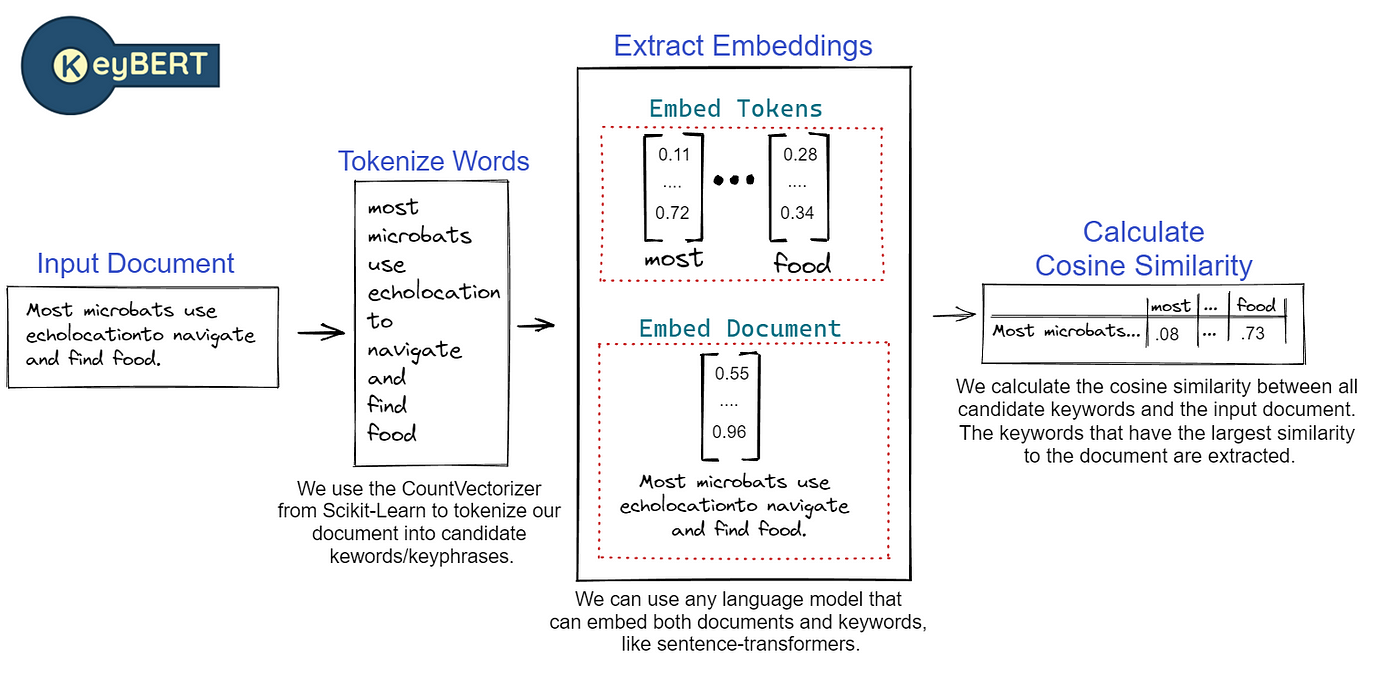
\includegraphics[width=80mm,scale=0.5]{pic/keybert.png}
    \caption{\textit{Pipeline} de la méthode \texttt{keybert} \citep{grootendorst2020keybert}.}
    \label{fig:enter-label}
\end{figure}
\end{frame}


\begin{frame}{\texttt{keybert} amélioré -- \textit{PatternRank}}
Key\textsc{BERT} + Keyphrase-Vectorizers = \textit{\textbf{PatternRank}} \hfill \citep{schopf2022}
\begin{itemize}
\item extraction des phrases-clés les plus similaires à un document
\item préservation de leur grammaticalité grâce aux motifs POS
\end{itemize}
\begin{figure}
    \centering
    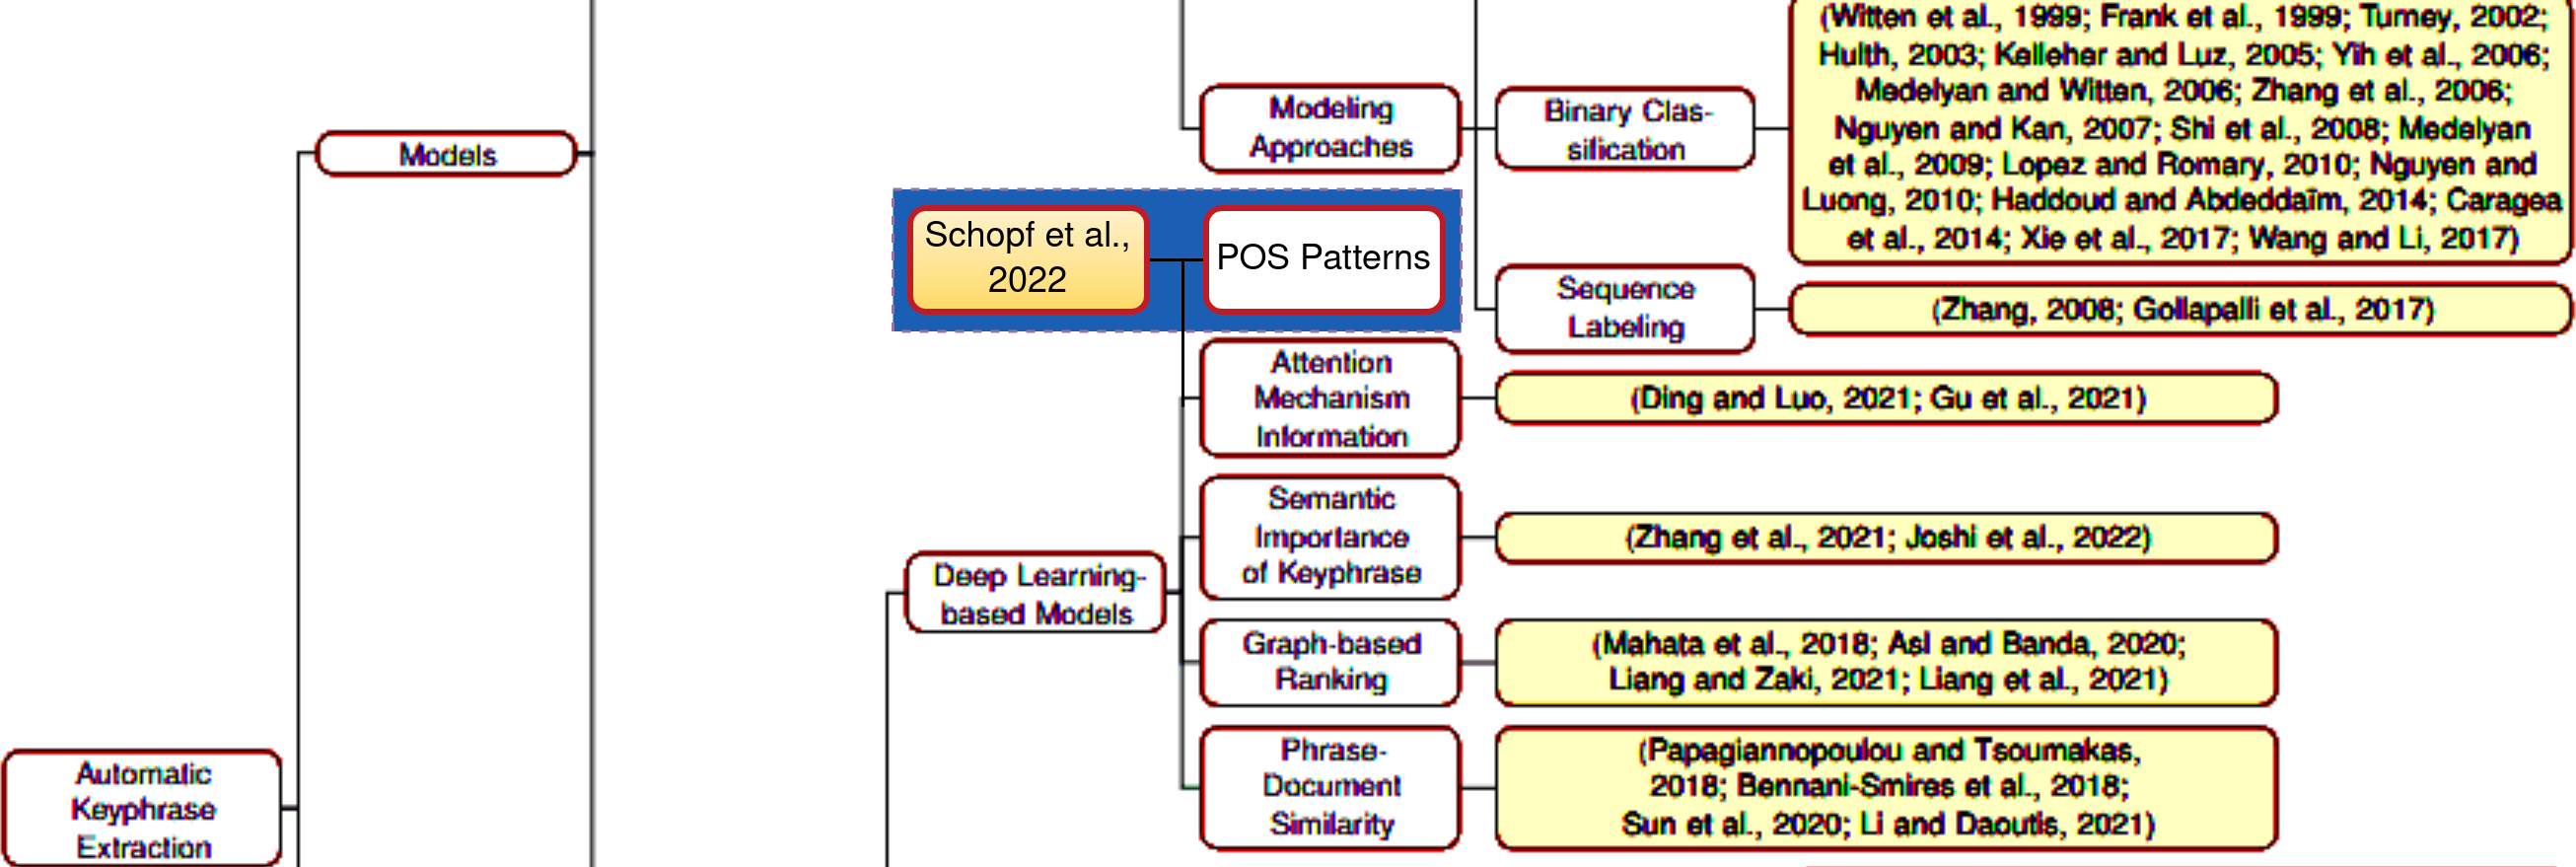
\includegraphics[width=110mm,scale=0.5]{pic/sota_lm_adapte.png}
    \caption{Extrait de l'état de l'art sur l'extraction des mots-clés, adapté de \citet{xie2023}}
    \label{fig:enter-label}
\end{figure}
\notecite{schopf2022}
\end{frame}

\begin{frame}{Fonctionnement de la méthode \textit{PatternRank}}
%\begin{itemize}
%\item extraction des phrases-clés non-supervisée
%\item exploite des modèles de langues pré-entraînés + parties du discours
%\end{itemize}
\begin{enumerate}
\item entrée : un seul document texte tokenisé
\item étiquetage des tokens avec les balises POS
\item sélection des tokens correspondant au modèle POS défini comme phrases-clés candidates
\item génération des plongements du document et des phrases-clés candidates par un modèle de langue
\item calcul des similarités cosinus entre les plongements du document et des phrases-clés candidates + classement des phrases-clés
\item extraction des \textit{N} phrases-clés les plus représentatives
\end{enumerate}
\begin{figure}
    \centering
    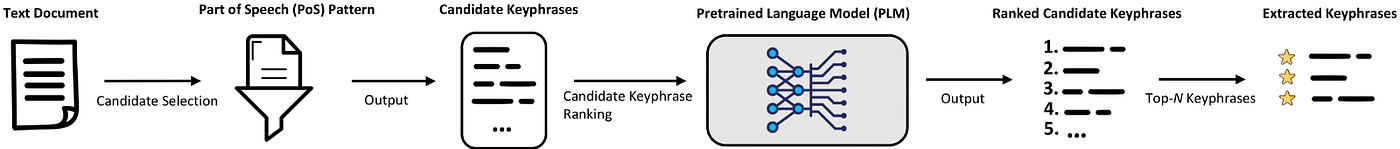
\includegraphics[width=110mm,scale=0.5]{pic/patternrank_workflow.png}
    \caption{\textit{Workflow} de la méthode \textit{PatternRank}.}
    \label{fig:enter-label}
\end{figure}
\end{frame}